Zaimplementowany~w~aplikacji sensor LVDT należy do grupy czujników wykorzystujących zmiany
parametrów obwodu -- indukcyjności. Czujnik typu LVDT (ang. \textit{Linear Variable Differential
  Transformer}, transformatorowy czujnik przemieszczeń liniowych) zbudowany jest na podstawie
transformatora różnicowego. Posiada on trzy uzwojenia -- pierwotne oraz dwa wtórne, które nawijane
są na cylindryczną, nieprzewodzącą obudowę. Wewnątrz obudowy znajduje się rdzeń ferromagnetyczny,
który może się swobodnie poruszać. Schemat układu przetwornika LVDT przedstawiono na
rysunku~\ref{img:lvdt}.

\begin{figure}[!htbp]
  \centering
  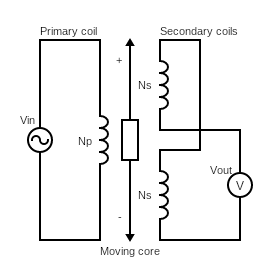
\includegraphics[width=0.4\textwidth]{sensor-theory/displacement-lvdt}
  \caption{\label{img:lvdt}Schemat układu przetwornika LVDT}
\end{figure}

Uzwojenie pierwotne zasilane jest napięciem przemiennym.~W~uzwojeniach wtórych (oznaczone jako Ns na
schemacie) indukują się napięcia, które zależne są od położenia rdzenia wewnątrz obudowy. Gdy rdzeń
znajduje się~w~równej odległości od obu cewek wtórnych -- napięcia będą sobie równe. Ponieważ układ
sensora LVDT jest zbudowany na podstawie transformatora różnicowego, to napięcie na wyjściu całego
układu będzie równe różnicy napięć na cewkach wtórnych. Zależność tę opisuje wzór
\cite{sensory_wykład}:

\begin{equation}
  u_{wy}=u_1-u_2=U_1 \sin{(\omega t + \varphi_1)} - U_2 \sin{(\omega t + \varphi_2)}
\end{equation}

Natomiast charakterystykę przetwarzania przetwonika LVDT (zależność napięcia wyjściowego oraz
przesunięcia rdzenia względem punktu równowagi) opisuje się wzorem:

\begin{equation}\label{eqn:theory-lvdt}
  U_{wy}=f\cdot I_p\cdot\bigg(4\pi\cdot N_p N_w\cdot \mu_0\cdot l_p\cdot\frac{x}{3l_w}\cdot
  \log{\Big(\frac{r_o}{r_i}\Big)}\bigg)\bigg(1-\frac{x^2}{2l_p^2}\bigg)
\end{equation}

\begin{eqparams}
  f & częstotliwość zasilania układu,\\
  I_p & prąd~w~uzwojeniu pierwotnym $I_p=\cfrac{U_{wej}}{R}$,\\
  N_p,\,N_w & liczba zwojów~w~uzwojeniach, odpowiednio~w~pierwotnym~i~wtórnych,\\
  l_p,\,l_w & długości uzwojeń, odpowiednio pierwotnego~i~wtórnych,\\
  \mu_0 & przenikalność magnetyczna próżni ($4\pi\cdot 10^{-7}$),\\
  x & przesunięcie rdzenia względem stanu ustalonego,\\
  \cfrac{r_o}{r_i} & stosunek promieni zewnętrzynych~i~wewnętrznych układu cewki,\\
\end{eqparams}

Charakterystyka przetwarzania sensora, przedstawiona na rysunku \ref{img:transfer-lvdt}, ma kształt
litery ,,V'', obie strony są symetryczne względem punktu zerowego -- stanu zrównoważenia. Dodatkowo,
napięcie wyjściowe nie jest zerowe~w~stanie równowagi -- jest to spowodowane niewielkimi różnicami
pomiędzy uzwojeniami wtórnymi \cite{sensory_wykład}.

\addimage{0.9}{sensor-theory/transfer-lvdt}{\label{img:transfer-lvdt}Przykładowa charakterystyka
  przetwarzania sensora LVDT~w~zależności od przesunięcia}

Sensory LVDT najczęściej stosuje się~w~zakresie $\pm$5 do $\pm$250mm, przy czym możliwe jest
mierzenie większych zakresach, jednakże wiąże się to ze znacznym zwiększeniem rozmiarów samego
przetwornika. Wykorzystanie przetwornika fazoczułego przy pomiarach przetwornikiem
LVDT pozwala na używanie jego pełnego zakresu, ponieważ możliwe jest określenie po której
stronie względem punktu równowagi znajduje się rdzeń. Napięcie wyjściowe z układu określa się wtedy
równianiem:

\begin{equation}
  U_{wy}=k\cdot{U_{wej}}\cdot\cos{(\varphi)}
\end{equation}

\begin{eqparams}
  k & współczynnik proporcjonalności,\\
  U_{wej} & napięcie wejściowe,\\
  \varphi & przesunięcie fazowe.
\end{eqparams}

Jeżeli napięcie wejściowe oraz wyjściowe będą w fazie, to kąt przesunięcia fazowego będzie
równy~0$^\circ$. Cosinus będzie wtedy równy 1. Natomiast w przeciwnej sytuacji (sygnały w
przeciwfazie), kąt $\varphi$ będzie równy 180$^\circ$, a cosinus będzie równy -1. Stosując
przetwornik fazoczuły przedstawiona powyżej charakterystyka przetwornika przyjmie postać
przedstawioną na rysunku \ref{img:transfer-lvdt-full}.

\addimage{0.9}{sensor-theory/transfer-lvdt-full}{\label{img:transfer-lvdt-full}Charakterystyka
  przetwarzania sensora LVDT po zastosowaniu przetwornika fazoczułego}

Sensory można stosować~w~dwóch typach układu: AC/AC oraz DC/DC.~W~przypadku układów
napięcia przemiennego otrzymuje się teoretycznie nieskończoną rozdzielczość pomiarową, większą
wytrzymałość mechaniczną przetwonika oraz mniejsze rozmiary układu. Natomiast korzystając~z~układów
napięcia stałego nie jest wymagane korzystanie~z~układów kondycjonujących sygnał oraz kompensujących
błędy pomiarowe. Częściej stosowane są jednak układy AC/AC~z~uwagi na zalety przeważające nad
układami DC/DC.
